%\documentclass[a4paper,11pt]{article}
\documentclass[final,3p,times,twocolumn]{elsarticle}
%\pdfoutput=1 % if your are submitting a pdflatex (i.e. if you have
             % images in pdf, png or jpg format)

%\usepackage{elsarticle} % for details on the use of the package, please
                     % see the JINST-author-manual

\usepackage[utf8]{inputenc}
\usepackage{textcomp}
\usepackage{lineno}
\usepackage{color}
\newcommand{\todo}[1]{\textcolor{red}{{#1}}}
\usepackage[outdir=./]{epstopdf}

%\title{\boldmath Commissioning and performance in beam tests of the highly granular SiW-ECAL technological prototype for the ILC}

% e-mail addresses: only for the forresponding author
%\ead{irles@lal.in2p3.fr}
%\collaboration[]{on behalf of the CALICE collaboration}

\begin{document}

\begin{frontmatter}
  \title{Beam test performance of the highly granular SiW-ECAL technological prototype for the ILC.}
  
\author{A. Irles}
    % e-mail addresses: only for the forresponding author
\ead{irles@lal.in2p3.fr}
%\collaboration[]{on behalf of the CALICE collaboration}


\begin{keyword}
  Calorimeter methods, calorimeters, Si and pad detectors
\end{keyword}

%\maketitle
%\flushbottom


\begin{abstract}
  High precision physics at future colliders as the International Linear Collider (ILC) require unprecedented high precision in the determination
  of the final state of the particles produced in the collissions
  The needed precision will be achieved thanks to the Particle Flow algorithms (PF) which require compact, highly granular and hermetic calorimeters systems.
  The Silicon-Tungsten Electromagnetic Calorimeter (SiW-ECAL) technological prototype
  design and R\&D is tailored to the baseline design of the ECAL of the International Large Detector (ILD) for the ILC.
  In this document we present and discuss the commissioning of the prototype
  and the performance of the device in a beam test carried at DESY in June 2017.
\end{abstract}

\end{frontmatter}

\linenumbers


\section{Introduction}

Future accelerator based particle physics experiments
require very precise and detailed reconstruction of the final states produced
in the beam collisions. A particular example is the next generation of $e^{+}e^{-}$
linear colliders such the ILC\cite{Behnke:2013xla,Baer:2013cma,Adolphsen:2013jya,Adolphsen:2013kya,Behnke:2013lya}.
This project will provide collisions of polarized beams with centre-of-mass energies ($c.m.e$) of 250 GeV - 1 TeV.
These collisions will be studied by two multipurpose detectors:
the International Large Detector (ILD) and the Silicon Detector (SiD)\cite{Behnke:2013lya}.
To meet the precision levels required by the ILC %or CLIC
physics goals,
new techniques relying on single particle separation to make possible the choice of the best information available
in the full detector to measure the energy of the final state objects have been developed.
These techniques are called Particle Flow (PF) techniques \cite{Brient:2002gh,Morgunov:2004ed,Sefkow:2015hna}
and allow to reduce the impact of the poor resolution of the calorimeter systems (compared with trackers) in the overall reconstruction.
The detectors optimized for PF algorithms have some requirements. In the case of calorimeters: highly granular, compact
and hermetic calorimeters. 
The CALICE collaboration is doing R\&D of highly granular calorimeters \cite{Sefkow:2015hna} 
for future linear colliders.

In this document we will focus in the description of the silicon-tungsten electromagnetic calorimeter,
SiW-ECAL, its commissioning and its performance in beam test.
The SiW-ECAL is the baseline choice for the ILD ECAL. It consists in a detector (in the barrel region) of 24 $X_{0}$ of thickness which corresponds to $\sim 1~\lambda_{I}$ (interaction length).
It has silicon (Si) as active material and tungsten (W) as absorber material.
The combination of Si and W choices  makes possible the design and construction
of a very compact calorimeter with highly granular and compact active layers.
It will consist of an alveolar structure of carbon fiber into which modules made of tungsten
plates and the active sensors will be inserted. The very-front-end (VFE) electronics will be
embedded in the SLABs. The silicon sensors will be segmented
in squared cells (or channels) of 5x5 mm: a total of $\sim 100$ million channels will constitute the ECAL for ILD.
The desired signal dynamic range in each channel goes from 0.5 MIP to 3000 MIPs.
To reduce overall power consumption, the SiW-ECAL will exploit the special bunch structure
foreseen for the ILC: the $e^{+}e^{-}$ bunchs trains will arrive within
acquisition windows of $\sim$ 1-2 ms width separated by $\sim$ 200 ms. During the idle time, the bias currents of the electronics will be shut down.
This technique is usually denominated power pulsing. In addition to this, to cope with the large amount of channels,
the calorimeters should work in self-trigger mode (each channel featuring an internal trigger decision chain) and zero suppression mode. 

\section{The SiW-ECAL technological prototype}

The first SiW-ECAL prototype was the so called SiW-ECAL physics prototype.
It was successfully tested at DESY, FNAL and CERN running in front of another prototype from the CALICE
collaboration, the analogue hadronic calorimeter AHCAL, delivering the proof of concept of the technollogy
and the PF calorimetry.
For the physics prototype, the VFE was placed outside the active area with no particular constraints in power consumption.
It consisted of 30 layers of Si as active material alternated with tungsten plates as absorber material.
The active layers were made of a matrix of 3x3 Si wafers of 500 $\mu$m thickness. Each of these wafers was segmented in matrices of
6x6 squared channels of 1x1 $cm^{2}$, allowing for density of 1500 channels/dm$^{3}$
The prototype was divided in 3 modules of 10 layers with different W depth per layer in each of these modules
(0.4, 1.6 and 2.4 $X_{0}$) making a total of 24 $X_{0}$.
That very first prototype offered a signal over noise on the measured charge of 7.5 for MIP like 
particles. More results proving the good performance of the technology and the PF can be found in
references~\cite{Adloff:2011ha,Anduze:2008hq,Adloff:2008aa,Adloff:2010xj,CALICE:2011aa,Bilki:2014uep}.

The new generation prototype is called the SiW-ECAL technological prototype. It addresses the main technological challenges: compactness,
power consumption reduction through power pulsing and VFE inside the detector close to real ILD conditions.
It will also provide data to deeply study the PF and provide input to tune simulation programs as for example
GEANT4\cite{Agostinelli:2002hh,Allison:2006ve,Allison:2016lfl} which is widely used
in particle physics to simulate the passage of particles through matter.


The entity
of sensors, thin PCB (printed circuit boards) and ASICs (application-specific integrated circuits)
is called Active Signal Units or ASU.
An individual ASU has a lateral dimension of 18x18 cm$^{2}$.
The ASUs are currently equipped
further with 16 SKIROC2\cite{}  (Silicon pin Kalorimeter Integrated ReadOut Chip)
ASICs for the read out and features 1024 square pads (64 per ASIC) of 5x5 mm.
The channels and ASICs are distributed along the ASU as shown in Figure \ref{ASU}.
Each ASU is equipped with 4 silicon wafers. The sensors consist on floating zone silicon wafers
320$\mu$m thick with high resistivity (bigger than 5000 $\Omega\cdot$cm).
The size of the wafer is $9\times9$ cm$^{2}$ and it is subdivided in an array of 256 PIN diodes of $5\times5$ mm$^{2}$.
A MIP (minimum ionizing particle) traversing the PIN parallel to its normal will create $\sim$ 80 $h^{+}e^{-}$ pairs per $\mu$m which corresponds to 4.1 fC
for particles incident perpendicularly to its surface.
The high voltage is delivered to the wafers using a high voltage kapton sheet that covers the full extension of the wafers.
The readout layers of the SiW-ECAL consist of a chain of Active Sensor Units (ASUs) and an adapter board
to a data acquisition system (DAQ) at the beginning of the layer.
The readout layers are embedded on a "U" shape carbon structure to protect the wafers.
The full system is then covered by two aluminum plates
to provide electromagnetic shielding and mechanical stability.
This ensemble is denominated SLAB
(``short'' for 1 ASU ensembles or ``long'' for several ASUs enchained) and it can be seen in
Figure \ref{ASU2}.
With current SLABs, a potential density of
4000 channels/dm$^{3}$ is achievable. This number should be compared with
the density achieved for previous beam tests: 1500 channels/dm$^{3}$ \cite{Amjad:2014tha}.

\begin{figure}[!t]
  \centering
    \includegraphics[width=0.4\textwidth]{../figs/test.jpg} 
  \caption{\todo{Temporary picture: La Esperanza del Condenado, J. Miró}: Open single SLAB with FEV11 ASU, 16 SKIROC 2, interface card and DIF visibles. }
\label{ASU2}
\end{figure}

\begin{figure}[!t]
  \centering
  \begin{tabular}{l}
    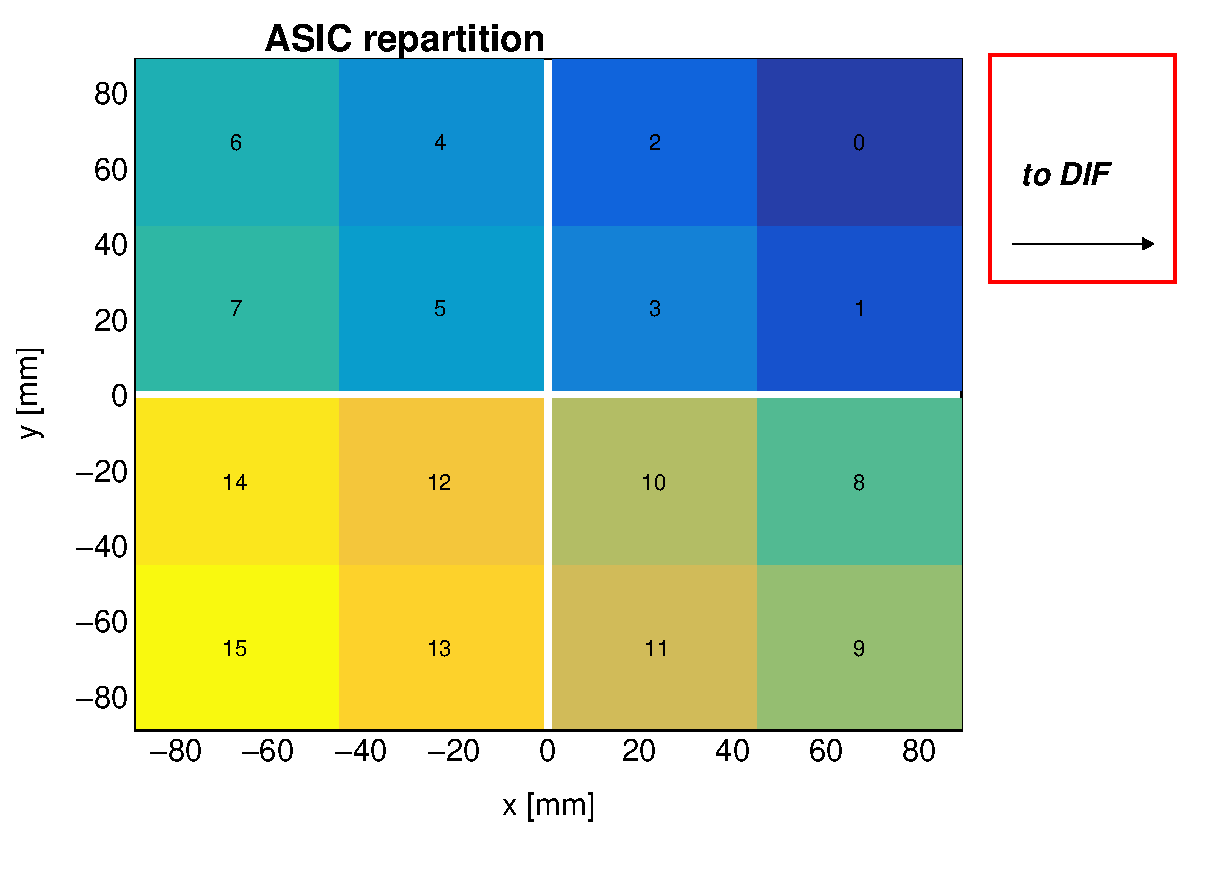
\includegraphics[width=0.4\textwidth]{../figs/ASU_geometry1.eps}  \\
    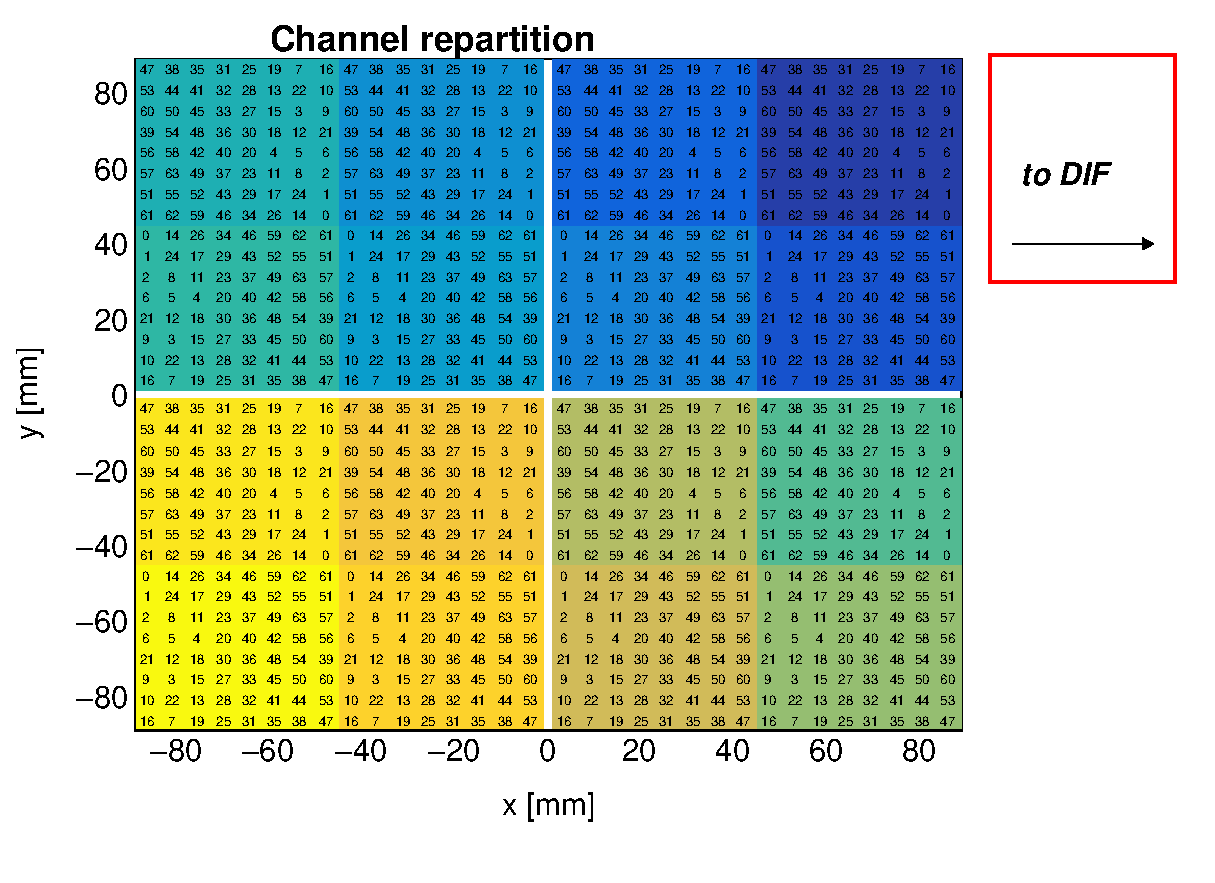
\includegraphics[width=0.4\textwidth]{../figs/ASU_geometry2.eps}  \\
  \end{tabular}
  \caption{Repartition of the ASIC (up) and channels (down) in one ASU. In this perspective, the Si-Sensors are in glued in the back.
    The channels are separated (in x and y) by 5.5 mm.
    The empty cross in the middle of the ASU corresponds to the 1 mm separation between the sensors.
    The areas covered by the different ASICs and channels
    are labeled with numbers following design and DAQ criteria: from 0-16 in the case of the ASICs and from 0-63 in the case of the channels.
  }
\label{ASU}
\end{figure}

The SiW-ECAL detector designed for the ILD requires of the order
of $10^{5}$ highly integrated detection like the ones described in this text.
For the production of the small sample of SLABs studied in this document,
a scalable working procedure has been established among several groups \cite{Boudry:2318814}
profiting from the funding of projects like AIDA2020 or the HIGHTEC emblematic project
of the P2IO.

The subsequent chain of the data acquisition (DAQ) system \cite{Gastaldi:2014vaa} is inspired by the ILC.
It consists on three layers of modules.
The first layer, or most downstream layer, consists on a set of detector interfaces called DIFs which are placed at the beginning of each SLAB holding up to 15 ASUs.
The second layer is made of concentrator cards module called the Gigabit Concentrator Cards (GDCCs)
which are used to control up to 7 DIFs collecting all data from them and distributing among them the system clock and fast commands.
The last layer consist on a clock and control card (CCC) which
provides a clock, control fan-out of up to 8 GDCCs and accepts and distributes external signals (i.e. signals
generated external pulse generator to simulate the ILC spill conditions).
The whole system is controlled by the Calicoes and the Pyrame DAQ software version 3~\cite{Rubio-Roy:2017ere,Magniette:2018wdz}.

\begin{figure}[!t]
\centering
\begin{tabular}{l}
\includegraphics[width=0.4\textwidth]{../figs/proto.png} 
\end{tabular}
\caption{Prototype with 7 layers inside the aluminum stack.}
\label{proto}
\end{figure}

A photograph showing the SiW-ECAL technollogical prototype setup can be seen in Figure \ref{proto}.
Current prototype consists on 7 layers of SLABs housed by a PVC and aluminum structure that can hold up to 10.
For the beam test described in Section \ref{sec:beamtest} all the layers were separated by equal distances of 15 mm
except the last one which was at 60 mm of its nearest. In the following sections, we will refer to layers number 1 to 7, where
the 1 is the closest to the beam pipe and 7 is the farthest.
The detector was exposed to a positron beam in the DESY test beam area (line 24).
During the full data taking period at the DESY beam test facility,
the detector was running in power pulsing mode without any extra active cooling system.
and means of an external pulse generator we defined the length of the acquisition window to be
3.7 ms at a frequency of 5 Hz.

\section{Performance on positron beam test at DESY}
\label{sec:beamtest}


The beam test line at DESY provides continuous positron beams in the energy range of 1 to 6 GeV with
rates from few hundreds of Hz to few KHz with a maximum of $\sim 3$ KHz for 2-3 GeV. 
The particles beam ies produced as follows: first, the electron/positron synchrotron DORIS II 
is used to produced a photon beam via bremsstralhung when interacting with a carbon fiber target;
secondly, these photons are then converted to electron/positron pairs; 
and, finally, the beam energy is selected with dipole magnets and collimators. 
In addition, DESY gives acces to a bore 1 T solenoid, the PCMag.

The physics program of the beam test can be summarized in the following points:

\begin{enumerate}
\item Calibration without tungsten absorber using 3 GeV positrons acting as minimum ionizing particle (MIPs) directed to 81 position equally distributed over the modules.
\item Test in magnetic field up to 1 T using the PCMag. For this test a special PVC structure was
designed and produced to support one single SLAB.	
The purpose of such test was twofold: first to prove that the DAQ, all electronic devices and the 
mechanical consistency of the SLAB itself are able
to handle strong magnetic fields; 
second to check the quality of the data and the performance of the detector during the data taking when running
in a magnetic field.
\item Response to electrons of different energies with fully equipped detector, i.e. sensitive parts {\it and} W absorber, with three different repartitions of the absorber material:
\begin{itemize}
\item W-configuration 1: $0.6,1.2,1.8,2.4,3.6,4.8$ and $6.6~X_{0}$
\item W-configuration 2: $1.2,1.8,2.4,3.6,4.8,6.6$ and $8.4~X_{0}$
\item W-configuration 3: $1.8,2.4,3.6,4.8,6.6,8.4$ and $10.2~X_{0}$
\end{itemize}
\end{enumerate}

First reports on this beam test can be find in
Refs. \cite{Irles:2018uum,Irles:2018hcd}. In this paper we discuss in detail
the results of the pedestal, noise and MIP calibration in Section \ref{sec:calib}.
We also show the results on the pedestal and noise stability when running inside
a magnetic field in Section \ref{sec:magnet}. The study of the perfomance of the detector
for electromagnetic shower events will be covered in future publciations.

\subsection{Commissioning}
\label{sec:commissioning}

Earlier experiences with the SKIROC2 ASIC are reported in Refs. \cite{Amjad:2014tha,Suehara:2018mqk}). 
Internal SKIROC2 parameters found in these references are adopted in the following
except if the opposite is stated.
For example, the gain value of 1.2pF for the preamplifier is used. 
With this gain, the SKIROC2 ensures a linearity better than 90\% 
for 0.5-200 MIPs, which is enough for 
electromagnetic showers created by few GeV 
electrons or positrons.
This beam test was prepared by a careful and comprehensive commissioning comprising
the debug of the
short SLABSs with special emphasis in the control of the noise and the study of the
prototype performance in cosmic rays tests. Dedicated runs at the laboratory were taken
in order to identify and mask the noisy channels. The outcome of this study
is that X\% of the channels were masked before putting the detector in front of the beam.
Two different kinds of noisy channels were found: the ones that are noisy on all
SLABs and those which are only noisy in one or few of them. Preliminary inspections
of the PCB hints that the first group is associated to routing issues on the PCB and
hereafter they are labelled like this. The summary of this study is shown in Figure \ref{noisycells}.
These channels are removed from the data taking in all the studies shown from now on.

\begin{figure}[!t]
  \centering
  \begin{tabular}{l}
  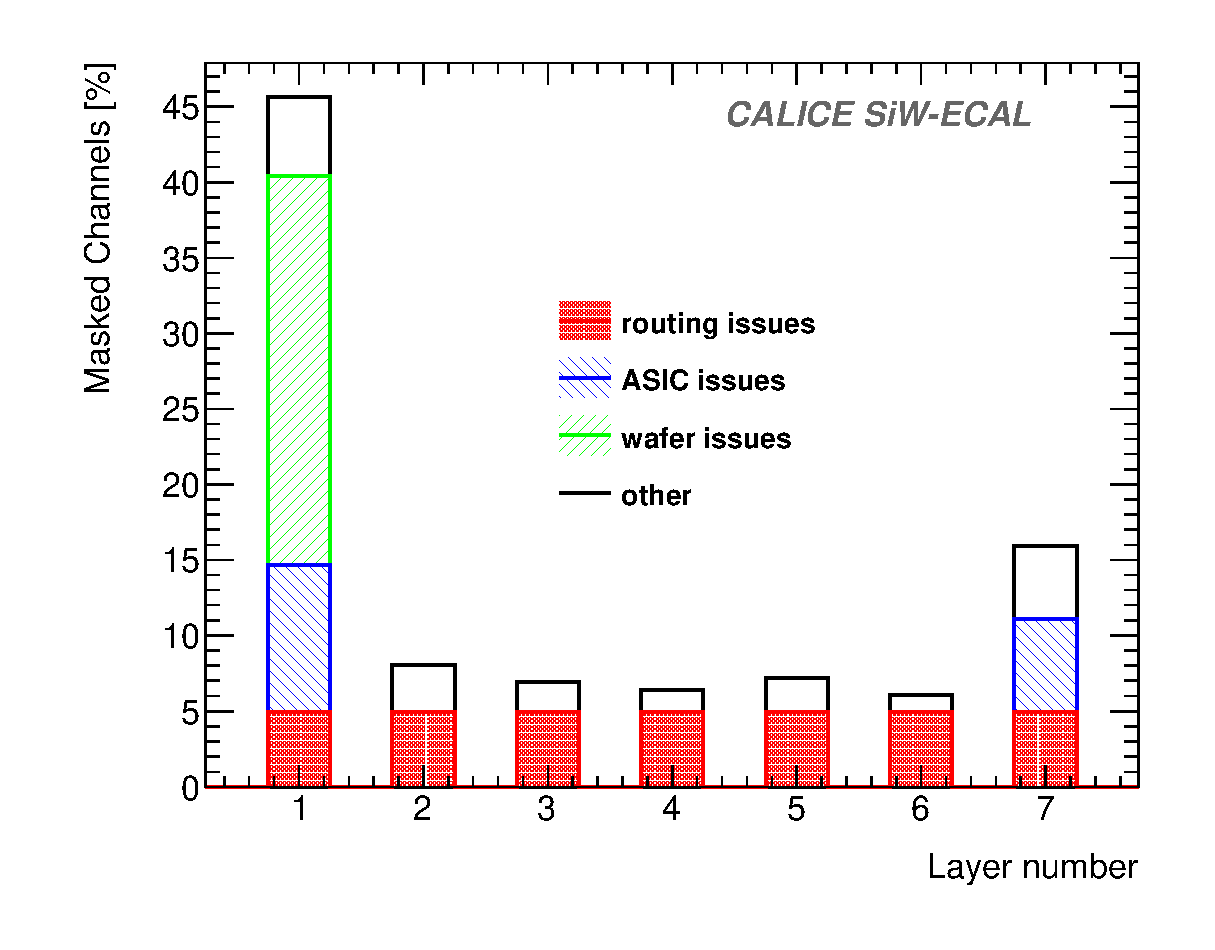
\includegraphics[width=0.4\textwidth]{../figs/commissioning/masked_layer.eps} \\
  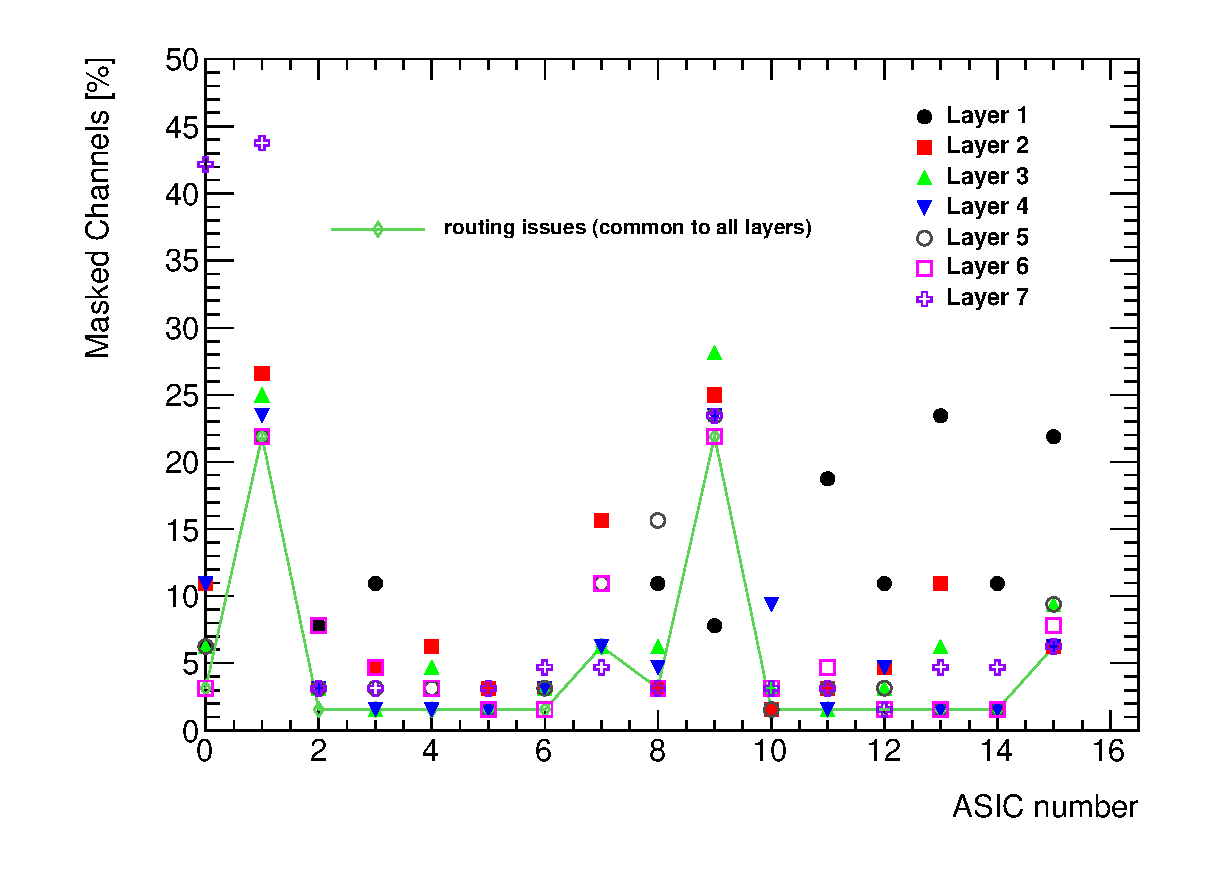
\includegraphics[width=0.4\textwidth]{../figs/commissioning/masked_chip.eps}
  \end{tabular}
\caption{Ratio of channels that are marked as noisy in all slabs. 
Top: inventory of the different type of noisy channels per slab. 
Bottom: break down of the total number of noisy channels per ASIC. 
The ASICs 4-7 (wafer issue) and 10 from layer 1 and the ASIC 4 from layer 7 are not included
in the second plot since they are fully masked.}
\label{noisycells}
\end{figure}

\subsubsection{Trigger threshold optimization}
\label{sec:comm_trigger}

\todo{Autotrigger stuf.
In order to select the optimal trigger threshold values for the detector operation
we perform dedicated scans of trigger threshold values
with all channels enabled (excepted the marked as noisy). }
The optimal trigger threshold values for all ASICs are shown in Figure \ref{trigger_thresholds}.

\begin{figure}[!t]
  \centering
  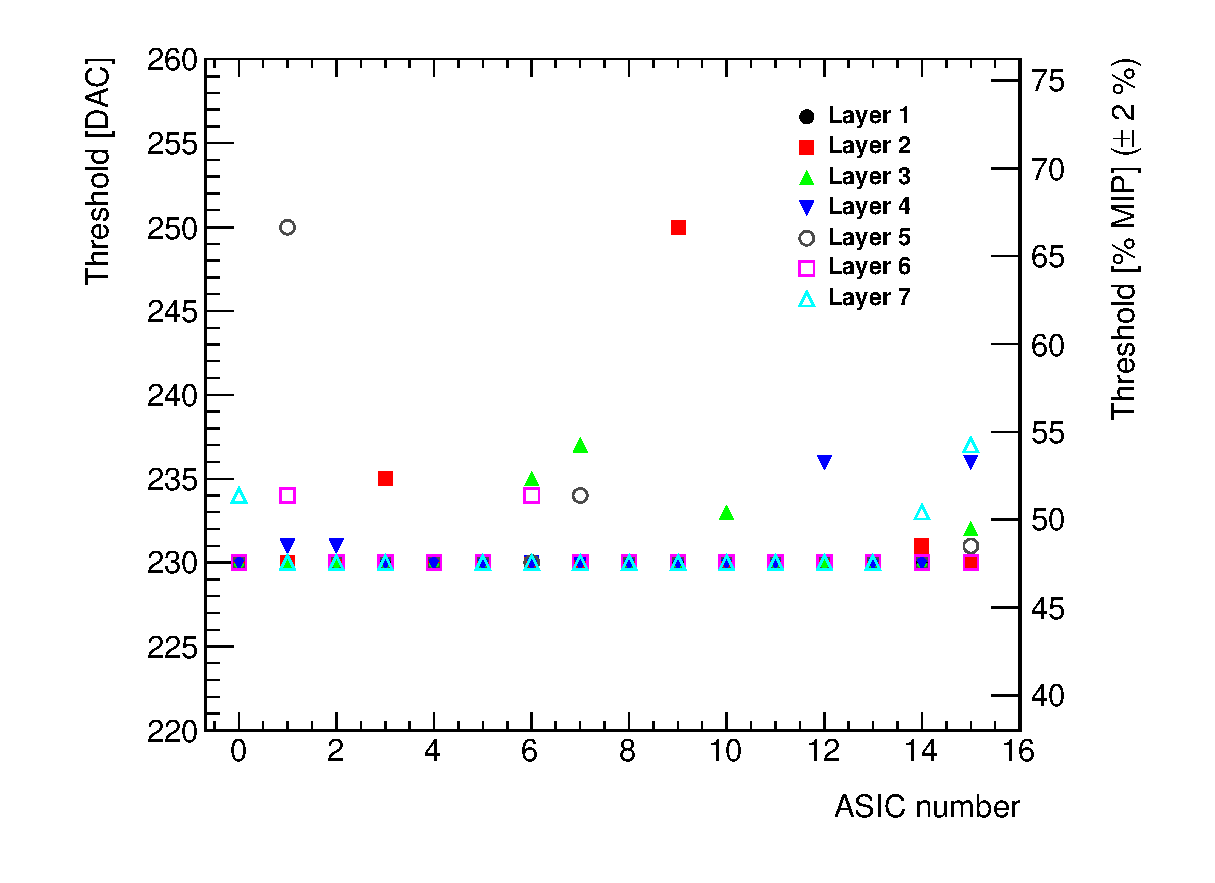
\includegraphics[width=0.4\textwidth]{../figs/commissioning/threshold_chip.eps}
  \caption{Summary of the trigger threshold settings in internal DAC units and in MIP units.}
\label{trigger_thresholds}
\end{figure}

\subsubsection{S/N ratio in the trigger line}
\label{sec:comm_trigger_sn}

In Figure \ref{scurves_injection} we see threshold scans curves
 curves obtained for several channel
in a SKIROC testboard in which a single SKIROC2 in BGA package is placed and the 1 MIP and 2 MIPs 
 signals are directly injected in the preamplifier 
(via a 3 pF capacitor located in the injection line as shown in Figure \ref{SKIROC2}). 
From this plot we can extract a S/N ratio of $\sim$12.8. 
Unfortunately, this results has obtained using
a dedicated board thought for commissioning and test of the SKIROC ASICS in an
"ideal" environment in contrast with the fully equipped
ASUS that are optimized to meet the detector requirement and to hold several ASICs at the same time.
We do not expect large differences with the results that we would obtain with 
a full equipped SLABs but dedicated runs in beam test will be needed.

\begin{figure}[!t]
    \centering
  \begin{tabular}{l}
	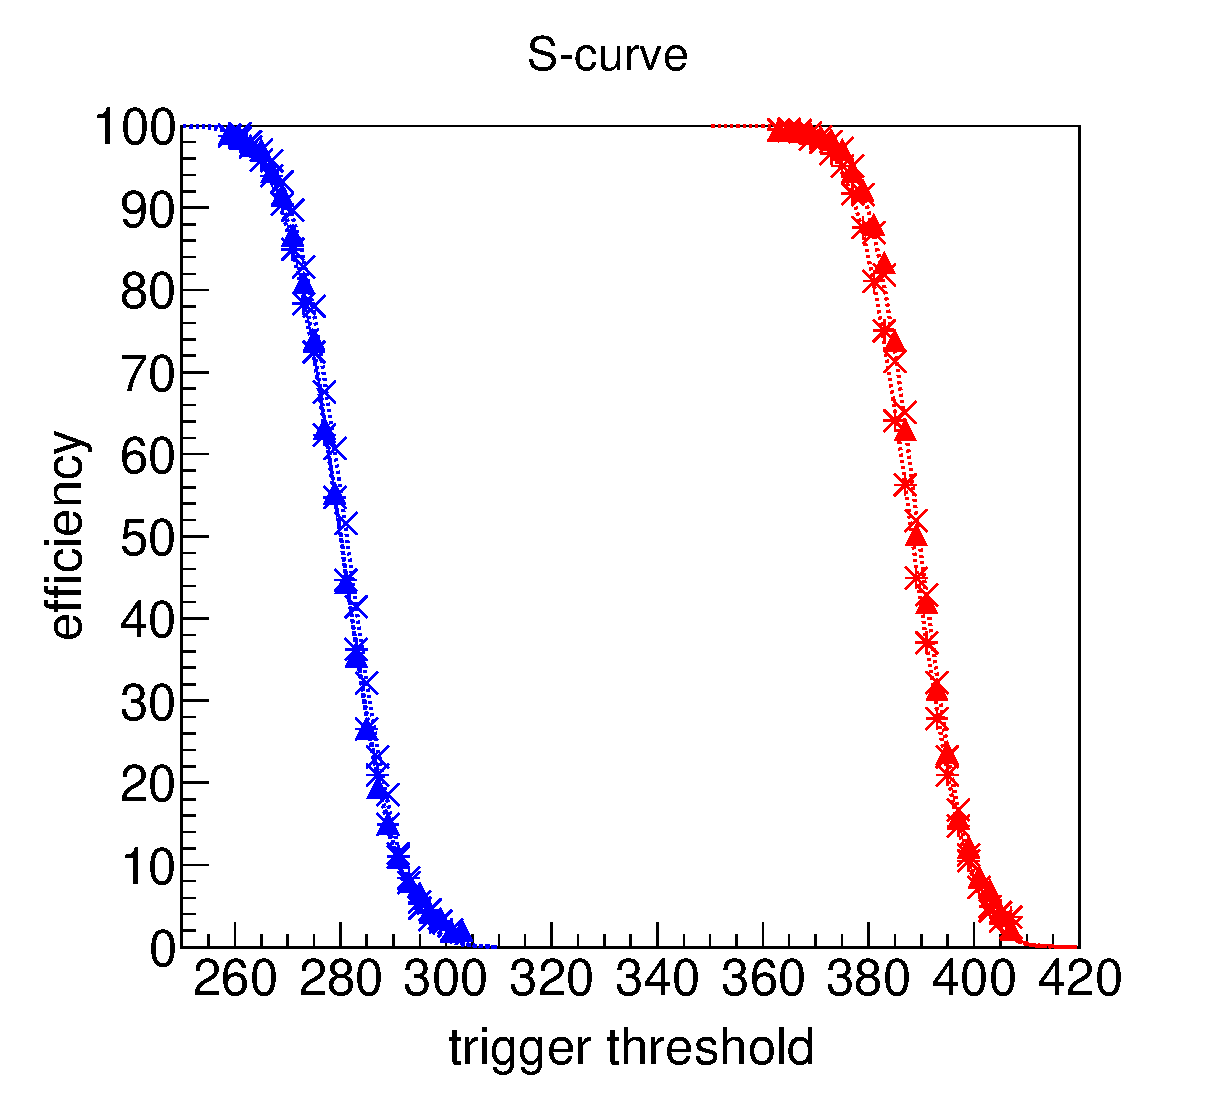
\includegraphics[width=0.4\textwidth]{../figs/commissioning/scurve_pp_fastshaper_ch.eps} \\
	\end{tabular}
\caption{Threshold curves with charge injection (1 MIP in blue and 2 MIPs in red) for two different channels in a SKIROC2 testboard. From this plot, we extract a $S/N = 12.8$ in the trigger line. \todo{We need to use charge in the axis}}
\label{scurves_injection}
\end{figure}


\subsection{Response to MIP-acting positrons}
\label{sec:calib}

\subsubsection{Pedestal and noise determination}
\label{sec:pedestal}

The calibration runs have been used to calculate the pedestal distribution reference values 
and the noise levels (the width of the pedestal distrution) of each channel.
In Figure \ref{signal_pedestal} we show the signal and pedestal distribution of a single channel after
subtracting the pedestal mean position. The results of the MIP calibration fit are included (red) and explained in the next version.
The pedestal distribution is shown only for the first SCA to keep the y-axis within a reasonable range.
The signal distribution is integrated over all SCAs.

\begin{figure}[!t]
  \centering
  \begin{tabular}{l}
    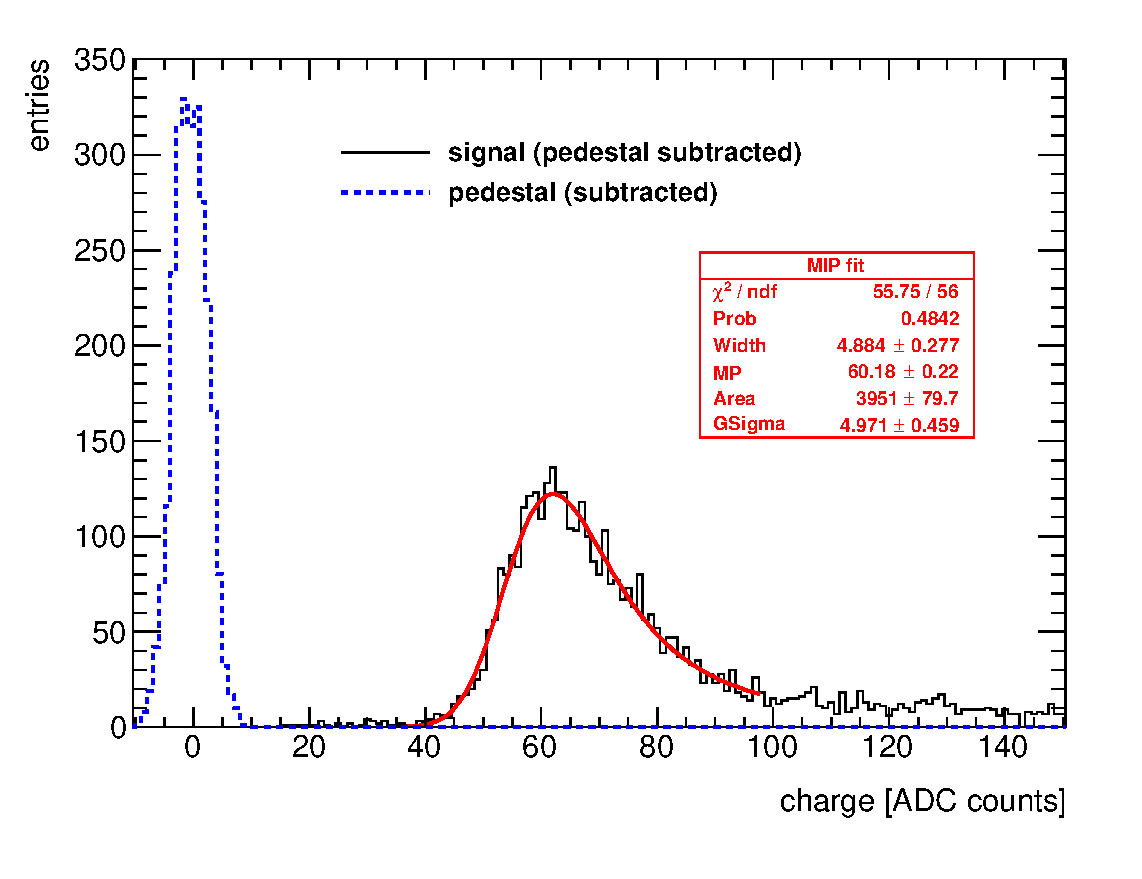
\includegraphics[width=0.4\textwidth]{../figs/mip_pedestal_example.eps}
  \end{tabular}
  \caption{Pedestal (blue dashed line) and signal (black continuous line) distribution for one channel in the third layer.}
\label{signal_pedestal}
\end{figure}

The pedestal is calculated as the mean position of
the ADC distribution of channels without trigger. The noise is
associated to the width of such distribution.
The pedestal correction is done layer-, chip-, channel- and SCA-wisely due to the large spread of values between pedestals, as observed in 
Figure \ref{pedestal_layer} (upper plot) and Figure \ref{pedestal_all} (also upper plot).
For the noise, the dispersion is much smaller ($\sim 5 \%$). This is shown in the lower plots of Figures \ref{pedestal_layer} and \ref{pedestal_all}.
From now on, the pedestal correction is applied to all the results presented.

\begin{figure}[!t]
  \centering
  \begin{tabular}{l}
    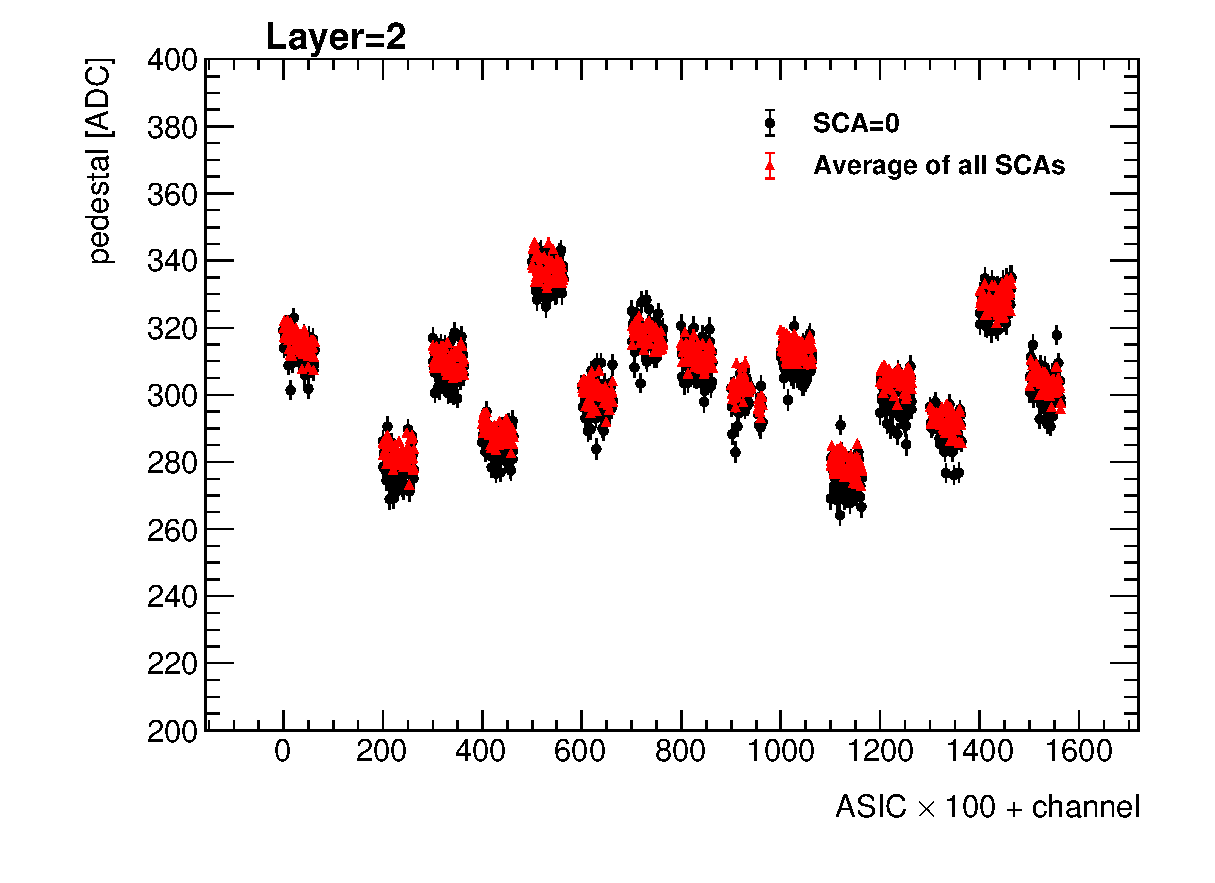
\includegraphics[width=0.4\textwidth]{../figs/pedestal/ped_mean_layer2.eps} \\
    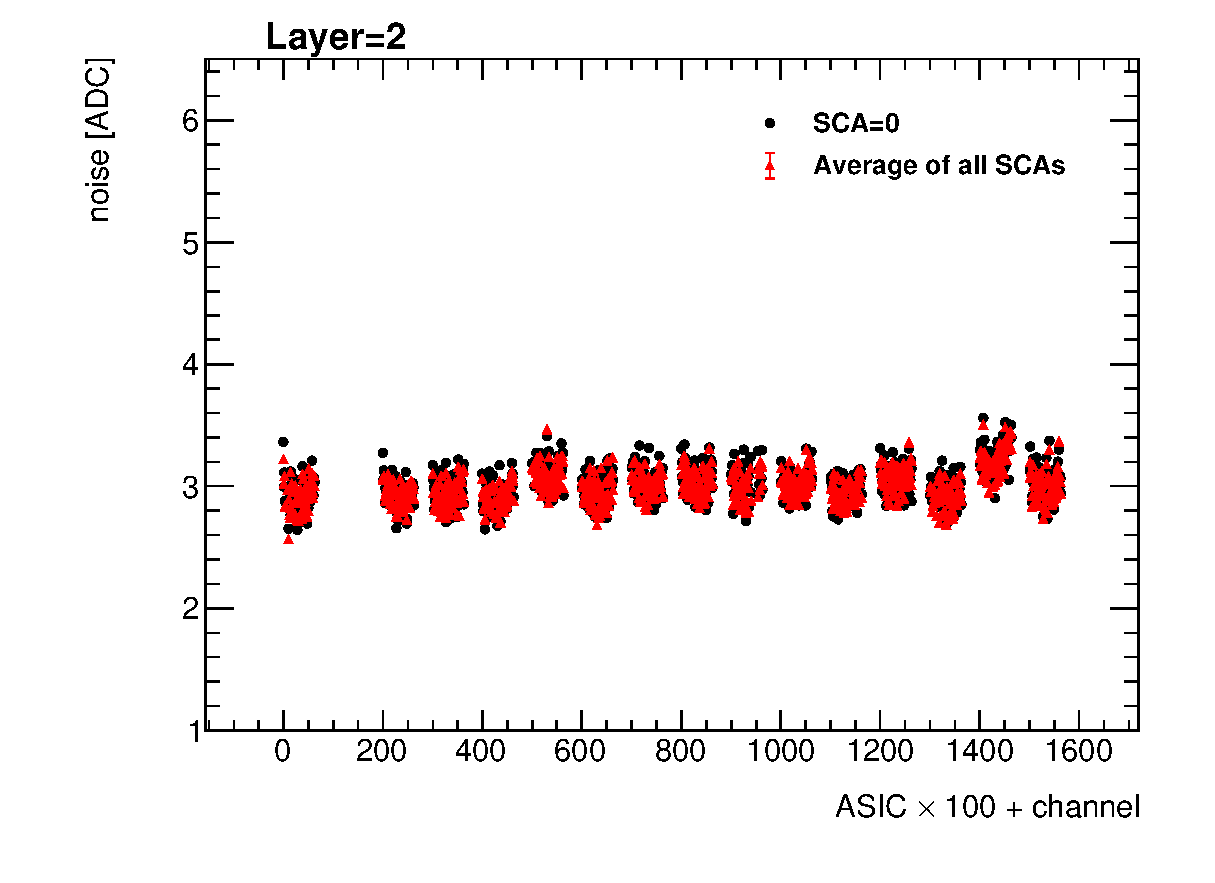
\includegraphics[width=0.4\textwidth]{../figs/pedestal/width_mean_layer2.eps}
  \end{tabular}
  \caption{Pedestal mean position (upper plot) and width (lower plot) for all channels in one layer. The data is grouped on bunches in which the value in the x-axis
    corresponds to the value of the channel number plus the value of the ASIC number multiplied by 100. The black points show the value for the first SCA
    and the red points show the average value for all the others SCAs (with the standard deviation of the sample as error bar).}
\label{pedestal_layer}
\end{figure}

\begin{figure}[!t]
  \centering
  \begin{tabular}{l}
    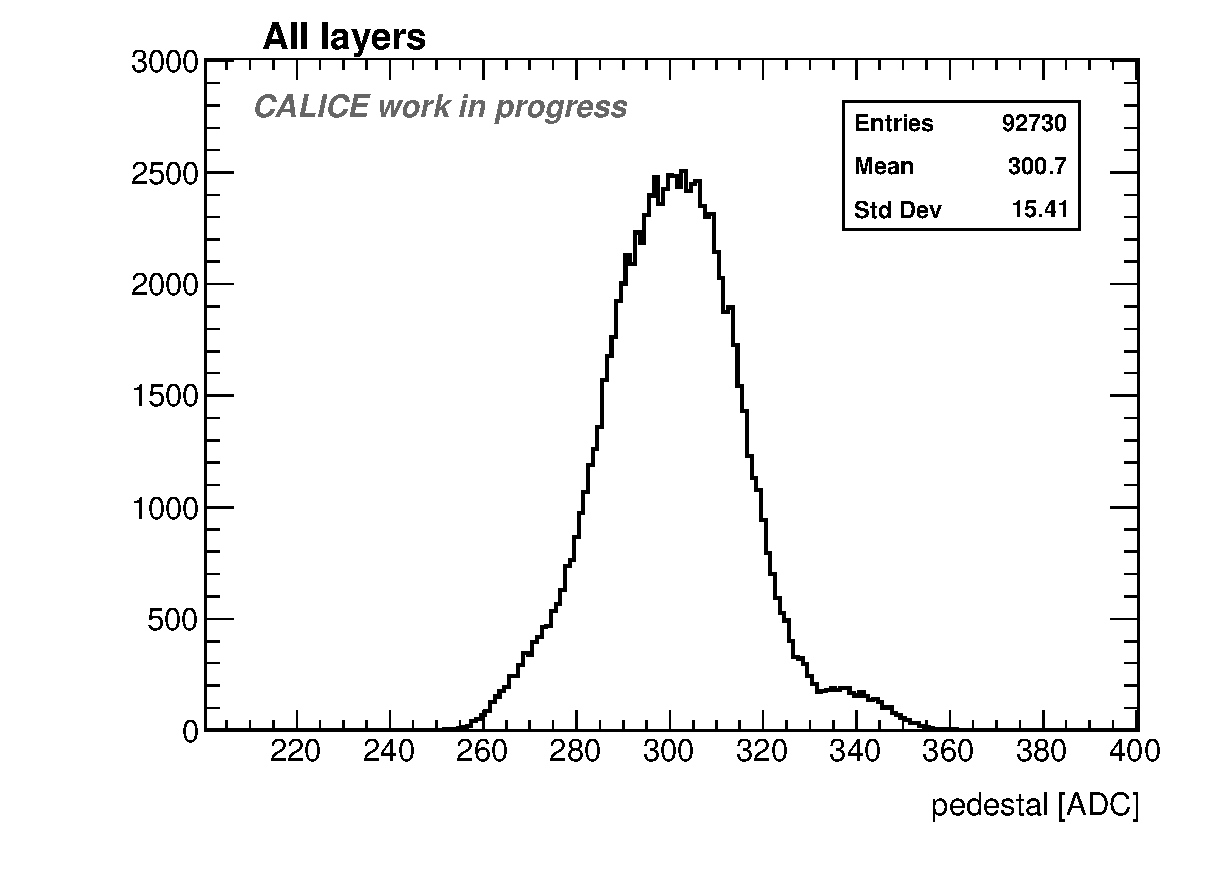
\includegraphics[width=0.4\textwidth]{../figs/pedestal/h_ped_mean.eps} \\
    \includegraphics[width=0.4\textwidth]{../figs/pedestal/h_ped_width.eps}
  \end{tabular}
  \caption{Pedestal mean position (upper) and width (lower) for all channels and all SCAs in the setup.}
\label{pedestal_all}
\end{figure}

\subsubsection{Energy calibration and tracking efficiency}
\label{sec:mip}

A Landau function convoluted with a Gaussian is fit to the resulting hit distribution. 
The most-probable-value of the convoluted function is taken as the MIP value, allowing thus for a direct
conversion from ADC units to energy in MIP units.
We have obtained a raw energy calibration spread of the 5\% among all channels with the 98\% of all 
available channels being fitted. Results are summarized in figure \ref{mipandSN}, upper plot.

\begin{figure}[!t]
  \centering
  \begin{tabular}{l}
    \includegraphics[width=0.4\textwidth]{../figs/MIP/MIPsummary_title.eps} \\
    \includegraphics[width=0.4\textwidth]{../figs/MIP/SNsummary_title.eps}  
  \end{tabular}
\caption{Result of the MIP position calculation and signal over noise calculation for all calibrated channels.}
\label{mipandSN}
\end{figure}

We checked the MIP 
calibration in all callibrated channels by selecting tracks
incident perpendicullary to the layers surface.
The results are shown in figure \ref{mip3peaks} where the single channel energy 
distribution for MIPs is shown for all calibrated channels in the same distribution. 
The maximum peaks at 1 MIP as expected after a good calibration.
In addition to this, a second and a third peak
appear visible. These peaks are due to
events involving multiple 
particles crossing the detector.

\begin{figure}[!t]
  \centering 
    \begin{tabular}{ll}
      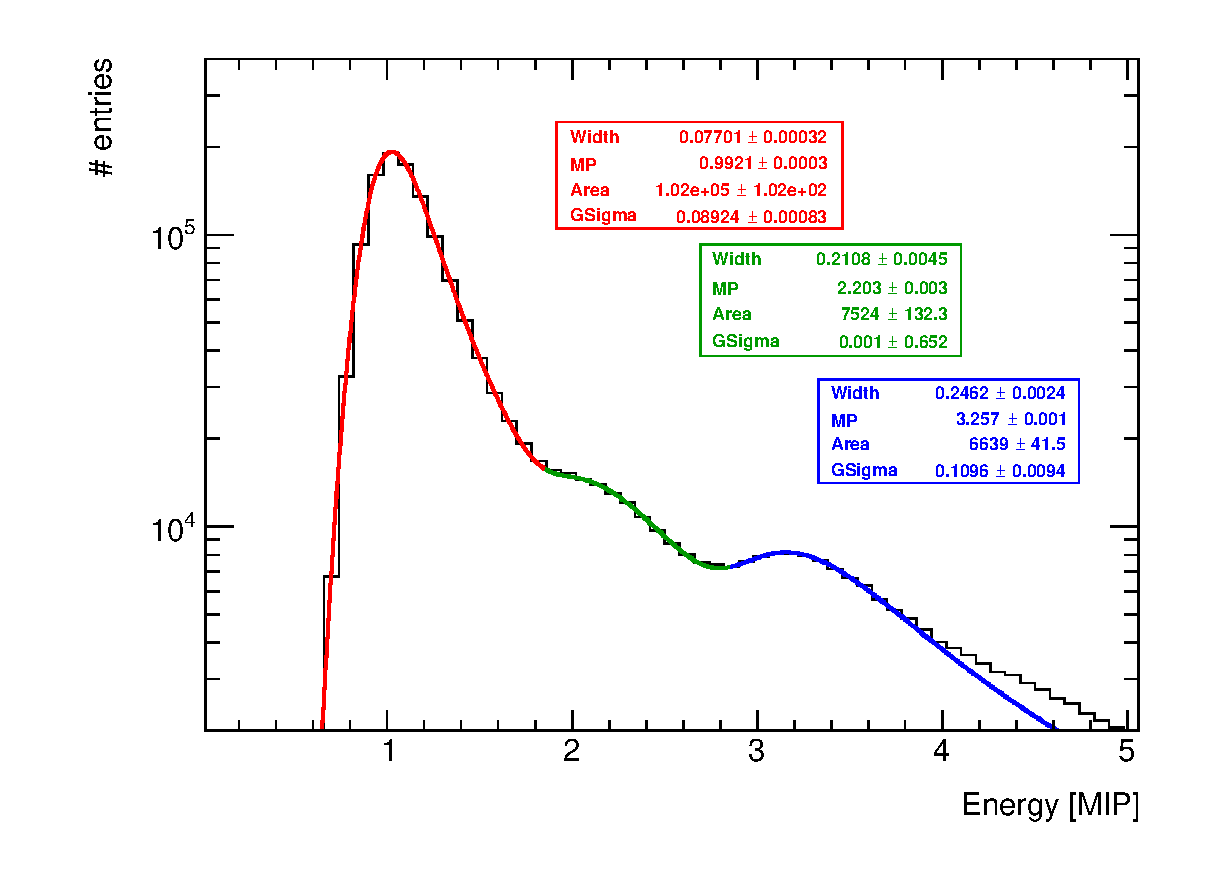
\includegraphics[width=0.4\textwidth]{../figs/MIP/MIP3peaks.eps} 
    \end{tabular}
    \caption{Energy distribution for all callibrated channels when selecting tracks of 3 GeV positron acting as MIPs.}
\label{mip3peaks}
\end{figure}

To evaluate 
the single hit detection efficiency we define a high purity sample of
events by selecting
tracks with at least 4 layers with a hit in exactly the same channel. Afterwards we 
check if the other layers have or not a hit in the same channel (expanding the search
to the closest neighbouring channels) with energy larger or equal than 0.3 MIP.
Finally, we repeat this for all layers 
and channels. The results are shown in Figure \ref{efficiency}. Except few exceptions, the efficiency is 
compatible with $100\%$.
Lower efficiencies in the first layer are related to the presence of
noisy channels not spotted during the commissioning. In the last layer (separated from the
other layers by four slots of 1.5 cm instead of only one) we also observe few small deviations
from the $\sim100\%$ which are indeed
associated to a slight misalignment of the detector.
If we remove these channels from the analysis
the full efficiency is recovered.

\begin{figure}[!t]
  \centering 
    \begin{tabular}{l}
      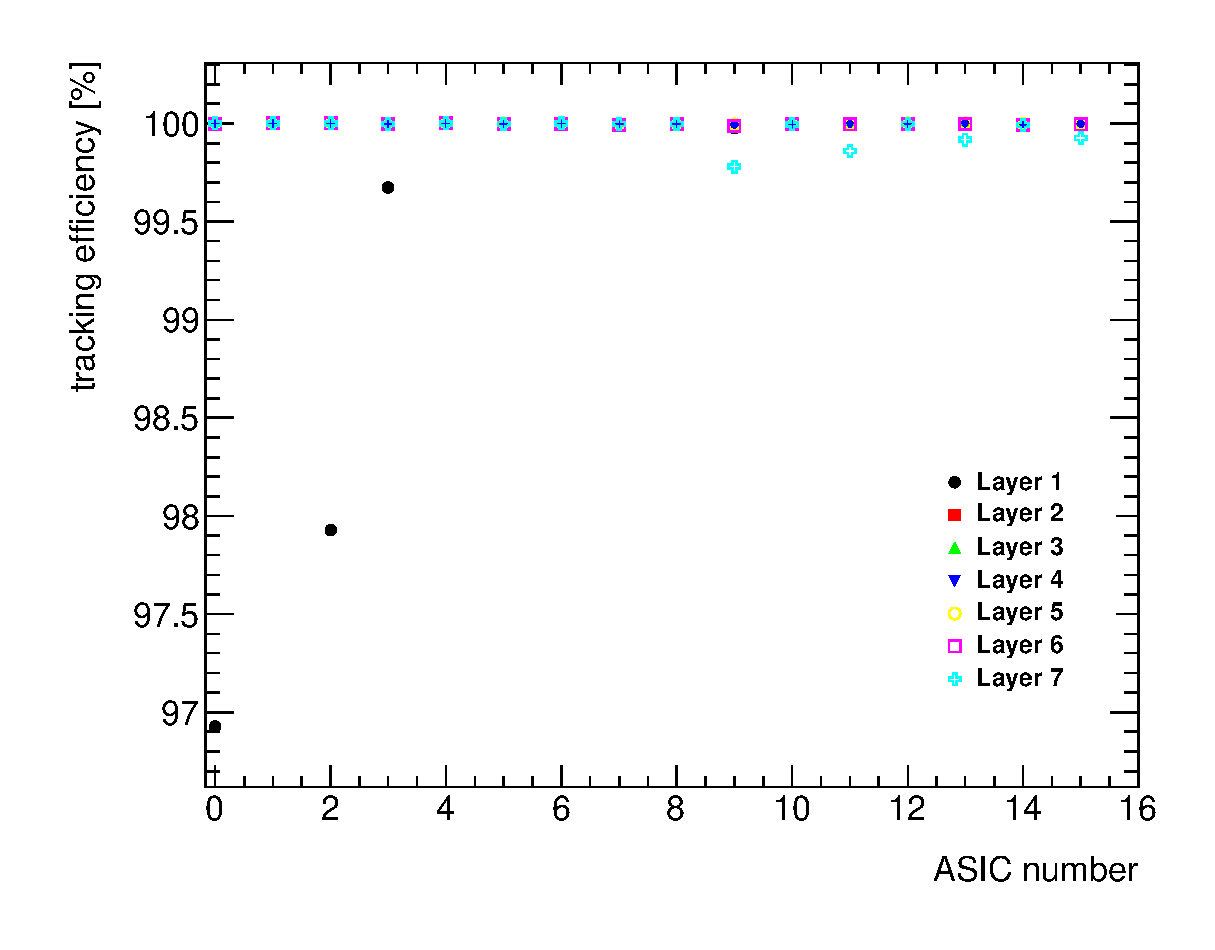
\includegraphics[width=0.4\textwidth]{../figs/MIP/efficiency_nhits4_chips.eps} \\
      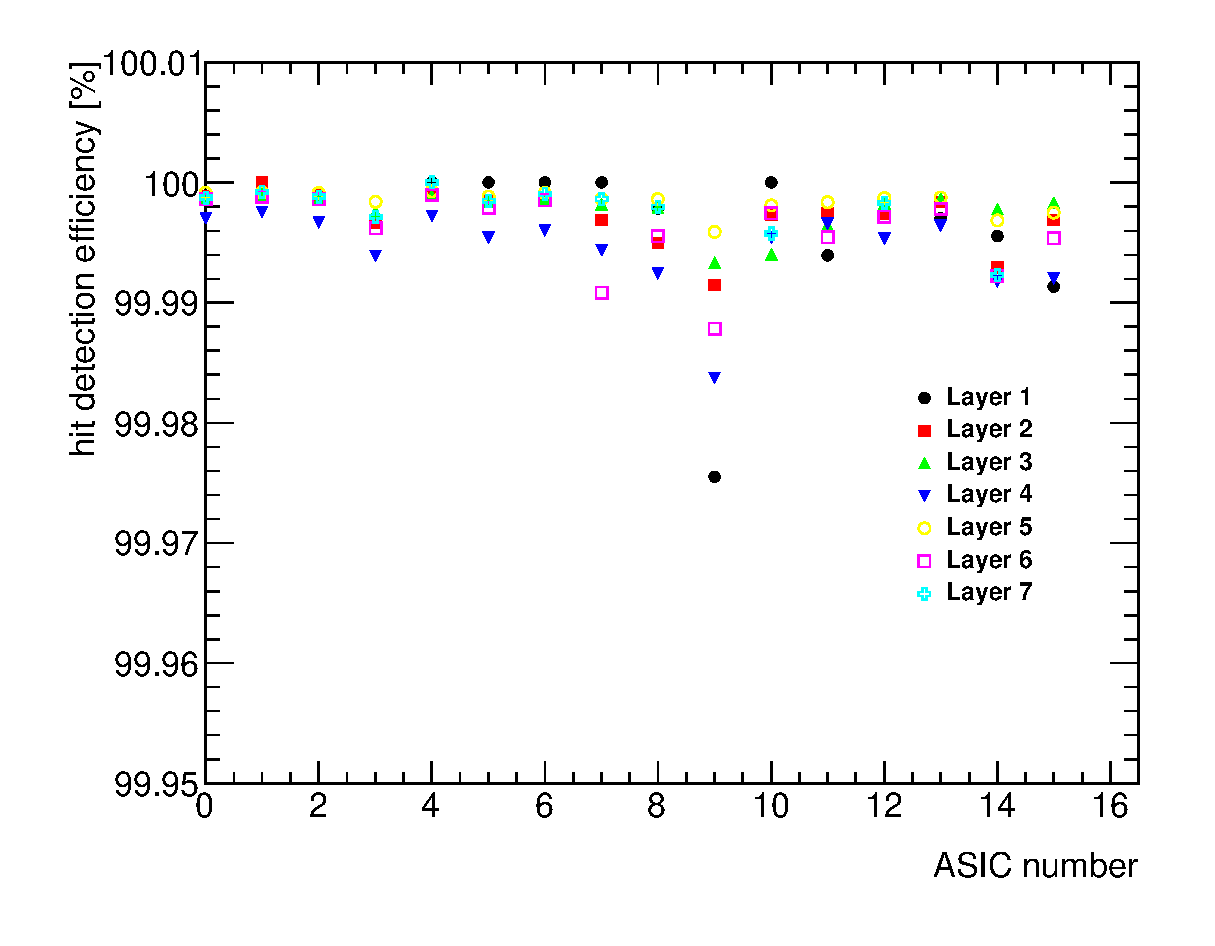
\includegraphics[width=0.4\textwidth]{../figs/MIP/efficiency_nhits4_chips_zoom.eps} 
    \end{tabular}
    \caption{Upper plot: MIP detection efficiency for all layers and ASICs in high purity samples of tracks of MIP-like acting particles. Lower plot: same figures with a zoom in the y-axis. In both cases, the average efficiency of the 64 channels in each ASIC is shown.}
\label{efficiency}
\end{figure}


\subsubsection{S/N ratio in the charge measurement for MIP interactions}
\label{sec:sn}

The signal-over-noise ratio in the charge measurement (corresponding to the slow shaper of the SKIROC2) is defined 
as the ratio between the most-probable-value of
the Landau-gauss function fit to the data (pedestal subtracted) and the noise (the pedestal width). This quantity 
has been calculated for all channels and all layers. The average S/N is to 20.4.
Results are summarized in Figure \ref{mipandSN}, rightmost plot.

\subsection{Pedestal and noise stability in a magnetic field}
\label{sec:magnetic}

The data taking inside the magnetic field has been divided in three steps:
a) a with a magnetic field of 1 T; b) a run with 0.5 T; c) a final run with the magnet off.
The beam, 3 GeV positrons, was hitting in the area of the PCB readout by the ASIC number 12.

The pedestal positions and noise levels of the channels of the ASIC 12 when the
SLAB is inside of the PCMag are compared with the results from the calibration run described in the previous section.
This is shown in Figure \ref{pedestal_magnetic}.
We see that the agreement is perfect within the statistical uncertainties.
Due to the lower rates in this beam area, the
analysis is only done up to few SCAs.

\begin{figure}[!t]
  \centering
  \begin{tabular}{l}
    \includegraphics[width=0.4\textwidth]{../figs/pedestal/1T/summary_pedestal_chip12.eps} \\
    \includegraphics[width=0.4\textwidth]{../figs/pedestal/1T/summary_noise_chip12.eps}
  \end{tabular}
  \caption{Average deviation of the pedestal mean position (left) and width (right) for all channels in the ASIC 12.}
\label{pedestal_magnetic}
\end{figure}

\section{Summary  and outlook}
\label{sec:summary}

The R\&D program of the highly granular SiW-ECAL detector is in an exciting phase. 
After the proof of principle of the imaging calorimetry concept using the physics prototype, the 
technological prototype is being constructed and tested. In this document we describe the commissioning and
beam test performance of a prototype built in with the first fully assembled
detector elements. In contrast with previous beam test, in this one we have fully
assembled detector elements meeting ILD requirements and the higher level of
density channel and total granularity achieved so far by this calorimeter.

A very comprehensive and detailed commissioning procedure has been established and optimized
allowing us to identify and isolate the different noise sources that could spoil the data taking.
The beam test has provided a lot of useful data to study 
the performance of the detector and  to perform
a channel by channel calibration.
A full analysis of the MIP calibration within magnetic field and
the response of the prototype in electromagnetic shower events
will be covered in a future document.

In parallel to the work described here, several R\&D efforts are being carried
and the results shown here are crucial for the next steps in the R\&D program.

One of these efforts is directed to the design and test of new ASICs.
In fact, a new generation of SKIROC2, the 2a, has been delivered
and it is being tested in the dedicated testboards and in a new generation of ASUs.
%In addition, a new generation of the ASIC, SKIROC3, is foreseen for the final detector construction.
%In contrast with SKIROC2/2a, the new ASIC will be fully optimized for ILC operaton, {\it i.e.} full zero suppression, reduced power consumption etc.

Many efforts are also concentrated in the construction and test of long SLABs
made of several ASUs enchained since we know that the ILD ECAL will host long layers of up to $\sim$2.5m.
This device constitutes a technological challenge in both aspects, the mechanical
(very thin and long structure with fragile sensors in the bottom, complicated assembly procedure...)
and the electrical (i.e. transmission of signals and high currents).
For example, interconnections between ASUs and between ASU and interface card are one of
the most involved parts of the assembly
and require close collaboration between mechanical and electronic engineers.
The construction and test of a long SLAB prototype
of $\sim8$ ASUs is currently ongoing.

In parallel to the ASUs equipped with BGA packaged ASICs, a different proposal for the ASU
design is being investigated. This is motivated by the high density of channels
demanded by the Particle Flow algorithms. Indeed, the FEV11 thickness is 1.6 alone and 2.7 mm
including the ASICs in its current packaging: 1.1 mm thick LFBGA package.
In this alternative PCB design the ASICs
are directly placed on board of the PCB in dedicated cavities.
The ASICS will be in semiconductor packaging and wire bonded to the PCB. This is the so-called COB (chip-on-board) version of the ASU.
A small sample of FEV11\_COBs (same connexion pattern with the interface card than FEV11)
with a total thickness of 1.2 mm allowing for a potential denisty of 10000 channels/dm$^{3}$ has been produced and tested in the laboratory
showing its readiness for tests with particle beams.% A sample can be seen in Figure \ref{cob}.
In addition, many efforts in the compactification of
the DAQ and the SLABs are currently being carried by the SiW-ECAL collaboration.

It is foreseen that all these developments, with the exception of the SKIROC3, will be tested with particle beams during 2018-2019.


\section*{acknowledgments}

This project has received funding from the European Union{\textquotesingle}s Horizon 2020 Research and Innovation program under Grant Agreement no. 654168.
This work was supported by the P2IO LabEx (ANR-10-LABX-0038), excellence project HIGHTEC,
in the framework {\textquotesingle}Investissements d{\textquotesingle}Avenir{\textquotesingle}
(ANR-11-IDEX-0003-01) managed by the French National Research Agency (ANR).
The research leading to these results has received funding from the People Programme (Marie
Curie Actions) of the European Union{\textquotesingle}s Seventh Framework Programme (FP7/2007-2013)
under REA grant agreement, PCOFUND-GA-2013-609102, through the PRESTIGE
programme coordinated by Campus France.
The measurements leading to these results have been performed at the Test Beam Facility at DESY Hamburg (Germany), a member of the Helmholtz Association (HGF).


%\bibliographystyle{JHEP}
\bibliographystyle{elsarticle-num}
\bibliography{../references}

\end{document}
